%!TEX program = lualatex
\documentclass[14pt]{constructor-thesis}

\usepackage[backend=bibtex]{biblatex}
\usepackage{tikz}
\usepackage{import}
\usepackage[mathscr]{euscript}
\usepackage{amsmath,amsthm,amssymb,latexsym,amsfonts}
\usepackage{thmtools}
\usepackage{lipsum}
\usepackage{soul}
\usepackage{amsmath,amssymb}
\usepackage{parskip}
\usepackage{graphicx}
\usepackage{mathtools}
\usepackage[usestackEOL]{stackengine}
\usepackage{tocloft}
\usepackage{xcolor}
\usepackage{hyperref}
\usepackage{tikz}
% \usepackage{pdfcomment}
% \usepackage{blindtext}
% \usepackage{todonotes}
\usepackage{hyphsubst}
\usepackage{bookmark}
\usepackage{pgfplots}
\usepackage{tikzsymbols}
\usepackage{cancel}
\usepackage{enumerate}
% \usepackage{wrapfig}
% \usepackage{graphicx}
\usepackage{extarrows}
\usepackage[bottom]{footmisc}
% \usepackage[table]{xcolor}
\addbibresource{thesis.bib}

\theoremstyle{definition}
\newtheorem*{theorem}{Theorem}
\newtheorem*{lemma}{Lemma}
\newtheorem*{definition}{Definition}

\newcommand{\pathstart}[1]{(#1)}
\newcommand{\pathhop}[3]{#1 \texttt{-[} #2 \texttt{]-} (#3)}

\newcommand{\patternstart}[1]{(#1)}
\newcommand{\patternhop}[3]{#1 \texttt{-[[} #2 \texttt{]]-} (#3)}

% \feetbelowfloat

\begin{document}
% Год, город, название университета и факультета предопределены,
% но можно и поменять.
% Если англоязычная титульная страница не нужна, то ее можно просто удалить.
\filltitle{en}{
  chair              = {Bachelor of Science \\ Computer Science},
  title              = {Mechanizing semantics of graph query languages in Coq},
  author             = {Semen Panenkov},
  supervisorPosition = {Prof.},
  supervisor         = {Anton Podkopaev},
  reviewerPosition   = {},
  reviewer           = {},
  chairHeadPosition  = {Dr.},
  chairHead          = {Stanislav Protasov},
}
\maketitle
\tableofcontents
% У введения нет номера главы
\section*{Introduction}

Databases have come a long way since their inception, and today we have a plethora of database types available, each designed to serve a particular use-case~\cite{database-types}. One of the more recent types to gain popularity are graph databases.

As the name suggests, graph databases represent data using graphs. While the idea of representing data with graphs isn't new with solutions developed as early as the mid-1960s, the first enterprise-ready ACID-compliant transactional database only emerged in 2007 with the release of Neo4j~\cite{enwiki:1146498781}. Since then, many graph databases such as Amazone Neptune, RedisGraph and NebulaGraph have sprung up~\cite{enwiki:1146498781}, with successful applications in various fields including recommendation services, fraud detection in finance~\cite{neo4j:use-cases} and even investigations of corruption schemes~\cite{icij:offshoreleaks}.

However, despite the growing popularity of graph databases, the lack of a standardized query language poses significant challenges to their wider adoption. The graph database community has developed Graph Query Language (GQL) to address this need. Nevertheless, standardizing GQL is challenging due to its complexity and constant expansion, and can result in errors and ambiguities even after thorough reviews~\cite{cpp-std-verified}. Furthermore, given the declarative nature of GQL, the database needs to determine how to fetch the data described in the query, leading to a greater number of possible implementations. This even poses into question the very existence of a realistic implementation.

% In fact, graph databases translate a query into an intermediate representation called \textbf{execution plan}, which is just a sequence of operations that need to be performed in order to evaluate the query. These operations inspect the graph and produce intermediate results that are later transformed by subsequent operations. This solution draws inspiration from relational databases world, where such approach has proven to be successful.

% However, this still leaves a lot of space to the implementators of the standard. For example, Neo4j and RedisGraph use different sets of operations and implement them differently. The former divides a query into a large sequence of small and simple operations while the latter covers with one complex operation the bigger part of a query but its operations are heavily optimized using linear algebra. The situation is further complicated by the fact that the translation process itself is complex and contains a lot of subtle details.

To address these challenges, we propose a formal approach to standardizing GQL and ensuring the correctness of the key details of query evaluation. Specifically, we aim to formalize the GQL semantics and demonstrate the correctness of the way that Neo4j and RedisGraph, our reference databases, translate queries to execution plans. To achieve this goal, we use the Coq proof assistant, a programming language that allows us to write and reason about programs with greater rigor and confidence. By providing a more robust approach to checking the correctness of the ecosystem around GQL, this work has the potential to contribute significantly to the wider adoption of graph databases.

% It allows to define mechanised, executable specifications whose correctness is machine-checkable.

% Competing graph databases typically use some dialect of the Cypher query language, much like how different relational databases use SQL. However, unlike SQL, there is no agreed-upon standard for Cypher. To address this, the graph database community developed Graph Query Language (or GQL), which is currently being standardized by ISO.

% This standard, like any other ISO standard, is just an informal human-readable text. Experience with other complex stardardized languages like C++ has shown that, despite the fact that such standards undergo a thorough review, they can still left some parts unspecified~\cite{cpp-std-verified} and even contain errors (citation needed about C++ memory model).

% Even if we concentrated all our efforts on correcting the current version of the standard, it would be impossible to maintain due to the fact that GQL is constantly being expanded.

% Moreover, proving that the standard is realistic and practical requires to actually implement the standard, i. e. to provide an evaluator of the GQL queries which complies with the standard.

% The situation is further complicated by the fact that GQL is a declarative language, meaning queries only describe what data is required, and the database has to figure out how to fetch it. This increases the number of possible implementations and may require us to introduce additional constructions to be able to evaluate the query. 

% In fact, graph databases translate a query into an intermediate representation called \textbf{execution plan}, which is just a sequence of operations that need to be performed in order to evaluate the query. These operations inspect the graph and produce intermediate results that are later transformed by subsequent operations. This solution draws inspiration from relational databases world, where such approach has proven to be successful.

% However, this still leaves a lot of space to the implementators of the standard. For example, Neo4j and RedisGraph use different sets of operations and implement them differently. The former divides a query into a large sequence of small and simple operations while the latter covers with one complex operation the bigger part of a query but its operations are heavily optimized using linear algebra.

% Moreover, the translation process itself is complex and contains a lot of subtle details.

% All of these notes imply that we need a more robust approach to check the correctness of all the parts that constitute the ecosystem around the currenly developed standard than just being careful.

% This is why we have decided to formalize the GQL standard and prove that the key details of the query evaluation are correct. Specifically, our aim is to demonstrate the correctness of the way that our reference databases, Neo4j and RedisGraph, translate queries to execution plans.

% To achieve that goal, we have chosen the Coq proof assistant which is basically a programming language that allows for writing and reasoning about programs.

\section{Related work}

There have been an attempt to mathematically formalize the standard~\cite{GQL-formalized-on-paper} which we used as a reference, however, this attempt is still pen-and-paper and, as a result, is prone to errors. In fact, we have identified some errors in the aforementioned paper.

% TODO: Describe the errors in the paper.

In contrast, there has been a successful attempt to formalize a subset of the SQL standard~\cite{sql-in-coq} and even write a verified relational database in Coq~\cite{rdbms-in-coq}. Their experience has shown that though many challenges remain, building fully-verified systems software in Coq is within reach.

\section{GQL and graph databases in a nutshell}

In this section we describe the basics of GQL and graph databases. For formal definitions we refer the reader to the paper about mathematical formalization of GQL~\cite{GQL-formalized-on-paper}. We assume some familiarity with SQL and relational databases.

\subsection{Property Graphs}
\label{section:intro-property-graphs}

Graph databases use so-called property graphs as an underlying data model. \textbf{A property graph} is a directed multigraph where each node\footnote{In the rest of the text we use words ``node'' and ``vertex'' interchangeably} or edge can store a possibly empty set of property-value pairs. To distinguish nodes and edges, each node and edge has a unique identifier\footnote{Even though any two vertex identifiers must differ as well as any two edge identifiers, sets of vertex and edge identifiers can overlap. They are considered to belong to different namespaces.}. In addition, labels can be added to nodes and edges to indicate their meaning.

\begin{figure}[b]
  \centering
  
  \import{img/}{property-graph.tex}

  \caption{Example property graph}
  \label{fig:property-graph}
\end{figure}

For instance, in figure~\ref{fig:property-graph} there are two nodes labelled ``Person'' and ``Company'' with identifiers 0 and 1, respectively. The company has a property ``name'' with a value of ``JB'', and there is an edge from the person to the company labelled ``WORKS\_FOR'' with id of 0. This edge also has a property ``since'' with a value of ``2022''.

\subsection{Values}
\label{section:intro-values}

In the subset of GQL we are interested in there are the following types of values:
\begin{itemize}
  \item \textbf{Graph object types.} Values of these types are vertex and edge identifiers.
  \item \textbf{Base types.} Values of these types are floating point numbers, integers and strings. 
  \item \textbf{Boolean type.} Values of this type are either \texttt{true}, \texttt{false} or \texttt{unknown}.
  % TODO: explain why we have `unknown` here.
\end{itemize}

Values of all of these types can be used in properties of graph objects.

\subsection{Binding tables}
\label{section:intro-binding-tables}

The result of a GQL query is represented with a so-called binding table which is analogous to the relation from SQL. Binding tables are also used to represent the intermidiate results during the query evaluation.

Basically, \textbf{a binding table} is a list of records. Each \textbf{record} is a tuple of values with named fields. \textbf{The domain of a record} is a set of all used names. \textbf{The type of a record} is a tuple with named fields of types of values under these names. A particular name-type pair is called \textbf{an attribute}. All the records in a table must have the same type, i.e. their domains must be the same and types of values under the same name must also match.

Because of the fact that all the records in any table have the same type, we can define \textbf{the type of a table} as the type of any of its records. An attribute of a record is also an attribute of the table.

\begin{table}
  \centering
  
  \begin{tabular}{ |p{3cm}|p{3cm}|p{3cm}|  }
    \hline
    \texttt{v : vertex} & \texttt{e : edge} & \texttt{u : vertex} \\
    \hline
    0 & 0 & 1 \\
    2 & 1 & 1 \\
    \hline
  \end{tabular}

  \caption{Example binding table}
  \label{tab:example-binding-table}
\end{table}

For example, in Table~\ref{tab:example-binding-table} there are two records and three attributes: \texttt{v : vertex}, \texttt{e : edge} and \texttt{u : vertex}. 


\subsection{GQL queries syntax and semantics}
\label{section:intro-GQL}

GQL queries consist of clauses, keywords and expressions like predicates and functions, many of which will be familiar to the users of SQL.


The following example query consists of three clauses:
\begin{verbatim}
MATCH (p:Person)-[e:WORKS_FOR]->(c:Company {"name": "JB"})
WHERE e.since >= 2020
RETURN *
\end{verbatim}

The first one is the \texttt{MATCH}-clause which allows to specify \textbf{a path pattern}. The result of this clause is a table where entries represent all the paths that match the pattern. The second clause is the \texttt{WHERE}-clause which allows to filter the records based on some predicate. And the last clause just says that we want to retrieve everything.

Let's dive deeply into the syntax of path patterns:
\begin{verbatim}
(p:Person)-[e:WORKS_FOR]->(c:Company {"name": "JB"})
\end{verbatim}

Here \verb+(p:Person)+ and \verb+(c:Company {"name": "JB"})+ are \textbf{vertex patterns} while \verb+-[e:WORKS_FOR]->+ is \textbf{an edge pattern}. \texttt{p}, \texttt{e}, \texttt{c} are vertex and edge pattern names. They are used to refer to the corresponding graph objects in the rest of the query. \texttt{Person} and \texttt{Company} are vertex labels. \texttt{WORKS\_FOR} is an edge label. \texttt{"name": "JB"} is \textbf{a property pattern}. It says that the company must have a property ``name'' with a value of ``JB''.

\begin{table}[b]
  \centering
  
  \begin{tabular}{ |p{3cm}|p{3cm}|p{3cm}|  }
    \hline
    \texttt{p : vertex} & \texttt{e : edge} & \texttt{c : vertex} \\
    \hline
    0 & 0 & 1 \\
    \hline
  \end{tabular}

  \caption{The result of the example query}
  \label{tab:example-query-binding-table}
\end{table}

Names of edge patterns are distinct and must differ from names of vertex patterns. However, names of vertex patterns can repeat. This can be used, for example, to look for cycles in the graph.

Names, labels and property patterns are optional. If a name is not specified, the matching graph objects are not listed in the result. For example, \texttt{()} is a completely valid vertex pattern.

The syntax \texttt{-[]->} says that the edge is directed from left to right, from the person to the company. We can also use \texttt{<-[]-} to match the edges in the reversed direction. And \texttt{-[]-} to say that the direction of the edge does not matter.

In the \texttt{WHERE}-clause the predicate \verb+e.since >= 2020+ says that the edge must have a property ``since'' with an integer value greater than or equal to 2020.

% TODO: grammar for the subset of GQL

If we run the example query on the example graph from Figure~\ref{fig:property-graph}, we will get the binding table~\ref{tab:example-query-binding-table}. This is because there is only one path in the graph that matches the pattern: $\pathhop{\pathstart{0}}{0}{1}$ (node 0 has the label \texttt{Person}, node 1 has a label \texttt{Company} and edge 0 has a label \texttt{WORKS\_FOR} and a property ``name'' with a value of ``JB''). Edge 0 also has a property ``since'' with a value of 2022 which is greater than 2020. So the predicate is true and the record is included in the result.

\subsection{Execution plans}

As you could see, GQL is a declarative language, meaning queries only describe what data is required, and the database has to figure out how to fetch it.

Like relational databases, graph databases translate a query into an intermediate representation called \textbf{an execution plan}, which is just a sequence of operations that need to be performed in order to evaluate the query. These operations inspect the graph and produce intermediate binding tables that are later transformed by subsequent operations.

Moreover, the optimization step of the query evaluation is usually performed on the execution plan of the query.

\begin{table}[t]
  \centering
  
  \begin{center}
    % \begin{tabular}{ |p{4cm}|p{11.5cm}|  }
    \begin{tabular}{ |c|l|  }
      \hline
      Name & \multicolumn{1}{c|}{Description} \\
      \hline
      \texttt{Expand(All)} & Traverses all edges from a given node. \\
      \texttt{Expand(Into)} & Traverses all edges between two nodes. \\
      \texttt{AllNodesScan} & Scans all nodes in the graph. \\
      \texttt{Filter} & Filters out rows that do not satisfy a given predicate. \\
      \texttt{ProduceResults} & Cleans up auxillary information. \\
      \hline
    \end{tabular}
    \caption{The most important execution plan operations for Neo4j}
  \end{center}
  \label{tab:execution-plan-operations-summary-Neo4j}
\end{table}
\begin{table}[t]
  \begin{center}
    % \begin{tabular}{ |p{4cm}|p{11.5cm}|  }
    \begin{tabular}{ |c|l|  }
      \hline
      Name & \multicolumn{1}{c|}{Description} \\
      \hline
      \texttt{Traverse} & Traverses paths that match the given pattern slice. \\
      \texttt{ScanNodes} & Scans all nodes in the graph. \\
      \texttt{Filter} & Filters out rows that do not satisfy a given predicate. \\
      \texttt{ReturnAll} & Cleans up auxillary information. \\
      \hline
    \end{tabular}
    \caption{The most important execution plan operations for RedisGraph}
  \end{center}
  \label{tab:execution-plan-operations-summary-RedisGraph}
\end{table}

Our reference databases, Neo4j and RedisGraph, use different sets of operations to evaluate queries. However, the general idea is the same. The tables~\ref{tab:execution-plan-operations-summary-Neo4j} and~\ref{tab:execution-plan-operations-summary-RedisGraph} show the most important operations for both databases.

\section{Goals and objectives}

Let us state our goal again. We want to mechanize the core subset of the GQL standard and its two main implementations in Coq.

To achieve this goal, we have set the following objectives:
\begin{itemize}
  \item \textbf{Mechanize the specification of the core subset of the GQL standard}:
  
  First, we want to write a specification for some subset of GQL. Our focus has been on read queries but GQL also allows for modifications. We have simplified the language by stripping away almost everything except path patterns. Our methodology is to start with a simple subset of the language and then expand it.

  We decided to provide the specification via denotational semantics. In other words, we describe which properties the resulting binding table should satisfy. This approach is very convenient for us because it allows us to write a specification in a very high-level way and treat the actual implementation of the specification later. However, this approach requires us to show that the specification is complete in some sense. We do this by proving that any two implementations of the specification are equivalent, i. e. for the same queries they produce equal binding tables up to permutations and repetitions of records.

  \item \textbf{Mechanize the specification of the execution plan}:
  
  Secondly, we want to specify some key operations of execution plans that are necessary to evaluate our queries. We decided to provide this specification via denotational semantics too. To achieve this, we have identified the crucial operations for Neo4j and RedisGraph and merged the operations that are common to both of them. Additionally, we have simplified the specification by omitting some details that are not relevant to our purposes.

  \item \textbf{Implement and prove the correctness of the translation of the queries}:
  
  The next objective is to define the translation from queries to execution plans and show that it is correct. Correctness in this case means that, according to the specification of the execution plan, the evaluation of translated queries satisfies the specification of GQL.

  % TODO: Show the scheme that explains what the correctness is.

  Neo4j and RedisGraph use different sets of operations and, thus, they translate queries differently. Therefore, we actually have to write two translators and prove their correctness separately.

  \item \textbf{Provide an example implementation of the execution plan evaluation}:
  
  It is also very important to implement those operations to prove that the specification we provided is realistic.
  
  Implementing almost all of the operations is pretty straightforward because they are simple enough. It is worth noting that we mostly aim to provide an implementation that just works. We are not trying to optimize the implementation for performance as it is out of the scope of this project.

  However, RedisGraph-specific \texttt{Traverse} operation is much more complex. Even though, we could implement it in a similar way as any other: making it just work, we decided that we want to capture the way RedisGraph implements it: using matrices. 
  
  % It has to translate a pattern slice into a complex matrix expression, evaluate the expression and iterate over the resulting matrix producing the resulting table. 

\end{itemize}

\section{Technical details}

In this section we describe the concrete definitions and theorems that we have proved as well as the ideas behind them.

\subsection{The specification of the core subset of GQL}

We start with the description of the core subset of GQL. We have chosen this subset because it is the simplest one that still reflects the main ideas of the language. We have also chosen this subset because it is the one that is used in the Neo4j and RedisGraph implementations.

\subsubsection{Values}

\begin{definition}
  We have the following \textbf{types} of \textbf{values} in our specification:
  \begin{itemize}
    \item \textbf{Graph object types.} Values of these types are vertex and edge identifiers. We denote the type of vertex identifiers by $\mathtt{vertex}$ and the type of edge identifiers by $\mathtt{edge}$.
    \item \textbf{Base types.} Values of these types are floating point numbers, integers and strings. We denote these types by $\mathtt{float}$, $\mathtt{int}$ and $\mathtt{string}$, respectively.
    \item \textbf{Boolean type.} Values of this type are either \texttt{true}, \texttt{false} or \texttt{unknown}. We denote this type by $\mathtt{bool}$.
  \end{itemize}
\end{definition}

\begin{definition}
  Given the value $v$ we can define the ``type of'' operator: $\mathtt{T}(v)$. It returns the type of the value $v$. For example, if we mean by $1$ an integer, then $\mathtt{T}(1) = \mathtt{int}$.
\end{definition}

\begin{definition}
  We can also define the typing relation for values. It is denoted by $v : t$ and means that the value $v$ has the type $t$. For example, $1 : \mathtt{int}$. Note that $v : t$ is equivalent to $\mathtt{T}(v) = t$.
\end{definition}

\subsubsection{Property graphs}

We start with the formal definition of property graphs. In short, a property graph is a directed labelled multigraph where each vertex or edge can store a possibly empty set of property-value pairs. 

\begin{definition}
  To begin we need to define some auxilliary terms: 
  \begin{itemize}
    \item \textbf{Vertex and edge identifiers} are positive integer numbers, i. e. $\mathbb{N}$.
    \item \textbf{Labels} are simply strings over some finite alphabet $\Sigma$. We denote the set of all labels that can ever be used by $L$, although it is just equal to $\Sigma^*$.
    \item \textbf{Properties} are represented as pairs of keys (plain strings) and values and are denoted by $P$.
  \end{itemize}
\end{definition}

\begin{definition}[Property graphs]
  We have chosen the following formal representation of property graphs:
  \begin{itemize}
    \item \textbf{Vertices and edges} are represented as finite sets of identifiers. We denote a set of vertices and a set of edges by $V$ and $E$, respectively. As mentioned earlier, these sets are not necessarily disjoint. Additionally, these sets can contain any numbers, however, we want these sets to be as close to $\{1 \dots |V|\}$ and $\{1 \dots |E|\}$ as possible. It is because we want to use these sets as indices in matrices. This way we can minimize the size of the matrices. Requiring that the sets are exactly of this form is, in practice, impossible if we take into account potential updates and deletions of vertices and edges.
    \item \textbf{Edge ends mapping function} denoted by $\eta$ is a function from $E$ to $V \times V$ which maps an edge to its ends. Note that with this definition all the edges are directed.
    \item \textbf{Labelling functions} are functions $\lambda_V : V \to 2^L$ and $\lambda_E : E \to L$ which map vertices and edges to their labels. Note that we use the powerset of labels for $\lambda_V$ because a vertex can have multiple labels. However, an edge can have one and only one label. The label of an edge is often called its \textit{type}. With this definition, we can say that a node $v$ or an edge $e$ has a label $l$ if $l \in \lambda_V(v)$ or $\lambda_E(e) = l$, respectively.
    \item \textbf{Properties mapping functions} are functions $\phi_V : V \to 2^P$ and $\phi_E : E \to 2^P$ which map vertices and edges to their properties. Note that we use the powerset of properties because a vertex or an edge can have multiple properties. However, we restrict those subsets to be finite.
    \item \textbf{A property graph} $G$ is, thus, a collection of all of those pieces. In other words, $G = (V, E, \eta, \lambda_V, \lambda_E, \phi_V, \phi_E)$.
  \end{itemize}
\end{definition}

For instance, the example graph on Figure~\ref{fig:property-graph} is represented as follows:

\begin{equation*}
  \begin{aligned}[t]
    V &= \{0, 1, 2 \} \\
    E &= \{0, 1, 2 \} \\
    \eta: & \\
          & 0 \mapsto (0, 1) \\
          & 1 \mapsto (0, 2) \\
          & 2 \mapsto (1, 2) \\
    \lambda_V: & \\
          & 0 \mapsto \{\texttt{Person}\} \\
          & 1 \mapsto \{\texttt{Company}\} \\
          & 2 \mapsto \{\texttt{Tech}\} \\
  \end{aligned}
  \qquad
  \begin{aligned}[t]
    \lambda_E: & \\
          & 0 \mapsto \texttt{WORKS\_FOR} \\
          & 1 \mapsto \texttt{LIKES} \\
          & 2 \mapsto \texttt{USES} \\
    \phi_V: & \\
          & 0 \mapsto \varnothing \\
          & 1 \mapsto \{(\texttt{``name''}, \, \texttt{``JB''})\} \\
          & 2 \mapsto \{(\texttt{``name''}, \, \texttt{``Coq''})\} \\
    \phi_E: & \\
          & 0 \mapsto \{(\texttt{``since''}, \, \texttt{2022})\} \\
          & 1 \mapsto  \varnothing \\
          & 2 \mapsto \varnothing
  \end{aligned}
\end{equation*}

\subsubsection{Binding tables}

\begin{definition}
  \textbf{A record} is a \textit{partial} mapping from names to values. We formally define names later.
\end{definition}

With this definition, we can ensure that we can't accidentally map the same name to two different values as opposed to defining a record as a set of pairs of names and values.

Note that we use the word \textit{partial} because we want to have records that don't use all the names. Formally, this means that a record is actually a total mapping from a subset of names.

Also note that with this definition, we can represent records with infinite domains, for example, $r(n) = 0$ for all $n$, although we will never construct such records.

The notation $(n \mapsto v)$ means that the name $n$ is mapped to the value $v$. For example, $(\mathtt{a} \mapsto 1)$ is a record that maps the name $\mathtt{a}$ to the value $1$.

\begin{definition}
  We can \textbf{update} the record $r$ by adding a new name-value pair $(n, v)$. We denote the updated record by $(n \mapsto v; r)$ and formally define it as:
  $$
  (n \mapsto v; r)(n') = \begin{cases}
    v & \text{if } n' = n \\
    r(n') & \text{otherwise}
  \end{cases}
  $$
\end{definition}

With these notations we can easily write down any record with a finite domain: $(n_1 \mapsto v_1; n_2 \mapsto v_2; n_3 \mapsto v_3)$.

\begin{definition}
  \textbf{The type of a record} $r$ is denoted by $T(r)$. $T(r)(n)$ is defined iff $r(n)$ is defined and $T(r)(n) = T(r(n))$.
\end{definition}

That is, the type of a record is a function that maps names to types of values stored under these names in the record. Moreover, we use the same notations for the types of records as for the records. For example, $T(n_1 \mapsto 1; n_2 \mapsto 2.0) = (n_1 \mapsto \mathtt{int}; n_2 \mapsto \mathtt{float})$.

\begin{definition}
  In the similar to values manner, we can define \textbf{the typing relation for records}:
  $$ r : T \Longleftrightarrow T(r) = T $$
\end{definition}

\begin{definition}
  \textbf{A binding table} is a set of some records.
\end{definition}

With this definition, we declare that we don't actually care about the order and number of repetitions of records in the table.

\begin{definition}
  We can define \textbf{the typing relation for binding tables}:
  $$ t : T \Longleftrightarrow \forall r \in t, \, r : T $$
\end{definition}

This definition implies that the binding tables in which records have different types don't have types. Moreover, the type is not unique. For example, empty binding table can have any type, although this is the only example. This will make sense later when we will show the specification for some execution plan operations. However, this means that we cannot define ``type of'' operator for all binding tables. Luckily, we won't actually need it.

\subsubsection{Patterns and paths}

Recall the example query from the section~\ref{section:intro-GQL}. As we previously discussed, the following part of the query is a path pattern:
\begin{verbatim}
  (p:Person)-[e:WORKS_FOR]->(c:Company {"name": "JB"})
\end{verbatim}

Here \verb+(p:Person)+ and \verb+(c:Company {"name": "JB"})+ are \textbf{vertex patterns} while \verb+-[e:WORKS_FOR]->+ is \textbf{an edge pattern}. We have discussed the exact syntax earlier.

% \texttt{p}, \texttt{e}, \texttt{c} are vertex and edge pattern names. They are used to refer to the corresponding graph objects in the rest of the query. \texttt{Person} and \texttt{Company} are vertex labels. \texttt{WORKS\_FOR} is an edge label. \texttt{"name": "JB"} is \textbf{a properties pattern}. It says that the company must have a property ``name'' with a value of ``JB''.

% \begin{definition}
%   \textbf{A vertex pattern} is denoted by $(n : l \, \{p_1: v_1, \ldots, p_k: v_k\})$ and \textbf{an edge pattern} is denoted by $\texttt{-[}n : l \; \{p_1: v_1, \ldots, p_k: v_k\}\texttt{]->}$ where $n$ is a name, $l$ is a label, and $p_i$ are property keys and $v_i$ are values. $(p_i, v_i)$ pairs consitute the properties pattern.

%   The syntax \texttt{-[]->} says that the edge is directed from left to right, from the person to the company. We can also use \texttt{<-[]-} to match the edges in the reversed direction. And \texttt{-[]-} to say that the direction of the edge does not matter.

%   Names, labels and property patterns are optional. For example, \texttt{()} is a completely valid vertex pattern.
% \end{definition}

\begin{definition}
  Formally, \textbf{a path pattern} is defined inductively:
  \begin{itemize}
    \item If $\pi_v$ is a vertex pattern, then $\patternstart{\pi_v}$ is a path pattern.
    \item If $\pi$ is a path pattern, $\pi_e$ is an edge pattern and $\pi_v$ is a vertex pattern, then $\patternhop{\pi}{\pi_e}{\pi_v}$ is a path pattern.
  \end{itemize}
\end{definition}

This notation of path patterns closely follows the actual syntax of GQL, however, it might appear confusing at first. You might think that $\texttt{-[[} \pi_e \texttt{]]-}$ means that the edge pattern is undirected but the information of the actual direction is contained in $\pi_e$. We use double brackets to emphasize that the direction is specified by the edge pattern itself.

\begin{definition}
  \textbf{A path} is defined inductively as well:
  \begin{itemize}
    \item If $v$ is a vertex, then $\pathstart{v}$ is a path.
    \item If $p$ is a path, $e$ is an edge and $v$ is a vertex, then $\pathhop{p}{e}{v}$ is a path.
  \end{itemize}
\end{definition}

The direction of $e$ is determined by the vertices adjacent to it. For example, if $e$ is an edge from $v_1$ to $v_2$, then in the path $\pathhop{\pathstart{v_1}}{e}{v_2}$ the the edge is directed from left to right while in the path $\pathhop{\pathstart{v_2}}{e}{v_1}$ the edge is directed from right to left.

Note that the paths are not necessarily simple. We can visit the same vertex or edge multiple times. For example, the path following path is valid:
$$\pathhop{\pathhop{\pathstart{v_1}}{e_1}{v_2}}{e_2}{v_1}$$

\subsubsection{Names}

We postponed the discussion of names until now because we needed to introduce the notion of a path pattern first. Now we can define them. As we mentined earlier, names in vertex and edge patterns can be omitted, however, they might be required during the intermidiate calculations. For example, the way that Neo4j evaluates the query requires names for all vertex and edge patterns to be present. 

Therefore, graph databases perform \textit{pattern normalization} before the actual query evaluation. This means that they add names to all vertex and edge patterns if they are missing. The names are generated automatically and are not visible to the user.

\begin{definition}
  To model that behaviour we define \textbf{a name} to be a string about which we know whether it is \textit{explicit} or \textit{implicit}. An explicit name is a name that is explicitly specified by the user. An implicit name is a name that is generated automatically by the database during the normalization process.
\end{definition}

This way, even though, the names can be omitted in the query, they are always present in the normalized query. So we can require that \textit{all} vertex and edge patterns have names in our specification, even though, some of them might be implicit.

\subsubsection{The pattern-matching predicate and matching modes}

Let's fix the property graph $G$ on which we operate. We can now informally define the pattern-matching predicate $\mathcal{M}$ as follows:

\begin{definition}
   A path $p$ with a record $r$ \textbf{matches} a pattern $\pi$ if and only if: $p$ matches $\pi$ and $r$ represents $p$. This is denoted as $\pi \models (p, r)$.
\end{definition}

The idea behind this definition is the following: it is convinient to define the pattern-matching using real paths in the graph. However, the output of a query is not a set of paths but a binding table. Therefore, we need to represent paths with records.

Informally defining what it means for a path to match a pattern is easy: the structure of the path must match the structure of the pattern, and vertices and edges must satisfy the requirements of the corresponding vertex and edge patterns. More concretely, the directions of the edges must match and vertices and edges must have the required labels and properties.

Representing paths with records is pretty easy too: an edge or a vertex of the path must appear in the record with the name specified in the corresponding vertex or edge pattern.

However, the path structure contains the full information about the path in the graph while in the resulting table we might not need all of it. For example, if the name in the original query was omitted (i. e. the name is implicit after normalization), the corresponding column in the resulting table should not appear. This is why we introduce the notion of the matching mode. It controls which names should appear in records.

\begin{definition}
  We have three \textbf{matching modes}:
  \begin{itemize}
    \item The \textit{full} mode means that all names should appear in the resulting records.
    \item The \textit{explicit} mode means that only explicit names should appear in the resulting records.
    \item The \textit{mixed} mode extends the explicit mode by allowing implicit names of vertex patterns that go after edge patterns with explicit names to appear in the resulting records. The usefulness of this mode will be explained later when we discuss the way RedisGraph translates patterns.
  \end{itemize} 
\end{definition}

This way, we can use, for example, the full mode during the query evaluation but require the explicit mode in the final result.

\begin{definition}
  We can denote the matching mode using the following notation:
  $ \pi \models_m (p, r) $
  where $m$ is either $F$, $E$ or $M$ standing for full, explicit and mixed matching modes respectively.
\end{definition}

We could weaken the definition of the pattern-matching predicate by relaxing such strict control of implicit names but this definition turned out to be very convinient during the rigorous proofs because having a stronger predicate means having stronger induction hypotheses.

\begin{definition}
  Using the matching mode $m$ we can define \textbf{the type of a pattern} $\pi$, denoted as $T_m(\pi)$, inductively by mirroring the structure of the pattern:
  \begin{itemize}
    \item If $\patternstart{\pi_v}$ is a pattern, $n_v$ is the name of $\pi_v$ and it should appear in the result according to the matching mode $m$ then $T_m \patternstart{\pi_v} = (n_v \mapsto \texttt{vertex})$. Otherwise, $T_m \patternstart{\pi_v}$ is empty.
    \item If $\patternhop{\pi}{\pi_e}{\pi_v}$ is a pattern, $n_v$ and $n_e$ are the names of $\pi_v$ and $\pi_e$ respectively, and they should appear in the result according to the matching mode $m$ then
    $$T_m(\patternhop{\pi}{\pi_e}{\pi_v}) = (n_v \mapsto \texttt{vertex}; n_e \mapsto \texttt{edge}; T_m(\pi))$$ 
    If any of these names should not appear in the result then we don't add it to the type.
  \end{itemize}
\end{definition}

We can notice that if the record matches the pattern then it has the record has the same type as the pattern. We can state this formally.
\begin{theorem}
  If $\pi \models_m (p, r)$ then $T(r) = T_m(\pi)$.
\end{theorem}
\begin{proof}
  By straightforward induction on the structure of the pattern.
\end{proof}

To transfer the records between the matching modes we can define the notion of explicit projections.

\begin{definition}
  \textbf{The explicit projection of a record} $r$, denoted by $r |_E$, is a record that contains only the explicit names from $r$. In other words, we narrow the domain of $r$ to explicit names only.

  Formally:
  $$ r|_E(n) :=
    \begin{cases}
      r(n) & \text{if $n$ is explicit} \\
      \text{undefined} & \text{otherwise}
    \end{cases} $$
\end{definition}

\begin{theorem}
  If $\pi \models_m (p, r)$ then $\pi \models_E (p, r |_E)$.
\end{theorem}
\begin{proof}
  By the definition of the pattern-matching predicate and the explicit projection.
\end{proof}

This theorem means that if we have a record that matches a pattern in any mode, we can easily obtain a record that matches the same pattern in the explicit mode. This is why we can use the explicit mode in the final result while using other modes during the query evaluation.

The converse is also true.
\begin{theorem}
  If $\pi \models_E (p, r)$ then there is $r'$ such that $\pi \models_m (p, r')$ and $r = r'|_E$.
\end{theorem}
\begin{proof}
  We can construct $r'$ because $p$ contains the full information.
\end{proof}

In a similar fashion we can define the explicit projection of a type.
\begin{definition}
  \textbf{The explicit projection of a type} $T$, denoted by $T |_E$, is a record that contains only the explicit names from $T$.
\end{definition}

Moreover, we can establish simple connections between the explicit projections of records and types.
\begin{theorem} If $r$ is a record and $\pi$ is a pattern, then:
  \begin{itemize}
    \item $T(r)|_E = T(r|_E)$
    \item $T_E(\pi) = (T_m(\pi)) |_E$
    \item $T_E(\pi) = T_E(\pi |_E)$
  \end{itemize}
\end{theorem}
\begin{proof}
  By the definitions.
\end{proof}

% TODO: describe the transitions between modes and explicit projections.

\subsubsection{The well-formedness of a pattern}

Not all patterns born equal. Some of them can be ill-constructed and cause a lot of trouble. For example, if some vertex and edge patterns share the same explicit name then the resulting records could not have both the matching vertices and matching edges. This is why we need to define the notion of the well-formedness of a pattern.

\begin{definition}
  \textbf{A pattern is well-formed} if the following is true about the names of its vertex and edge patterns:
  \begin{itemize}
    \item No vertex and edge pattern can have the same name.
    \item All implicit names are distinct.
    \item All edge names are distinct.
  \end{itemize}
\end{definition}

Note that an implicit and an explicit name are always considered distinct even if they share the same string. This is because the implicit names are tagged that they are implicit. So we can always distinguish explicit names from implicit.

Also note that the explicit vertex names may repeat. As we mentioned earlier, this allows us to look for cycles in the graph.

\subsubsection{The specification of GQL}

We can now specify the subset of the GQL language formally.
Again, by now we focus only on the path patterns. Therefore, all of our queries are of the form: $\texttt{MATCH} \; \pi \; \texttt{RETURN *}$ where $\pi$ is a path pattern. 

\begin{definition}
  \textbf{A query is well-formed} if its pattern is well-formed.
\end{definition}

\begin{definition}
  \textbf{The query evaluation function} $[ \cdot ]$ is a partial function from queries to binding tables. The $[q]$ is defined when the evaluation of $q$ succeeds and is equal to the resulting binding table.
\end{definition}

Note that the function is partial. For example, $[q]$ might not be defined if $q$ is not well-formed.

The specification of GQL turns out to be the specification of the query evaluation function.

Formally, we could specify it the following way:
\begin{align*}
  [\texttt{MATCH} \; \pi \; \texttt{RETURN *}] = \{ r \mid \exists p : \pi \models_E (p, r) \} \\ \text{ if $\pi$ is well-formed, otherwise undefined }
\end{align*} 

However, this definition requires us to check the well-formedness of the pattern and immediately reject ill-formed queries. This validation is tedious and is out of the scope of this thesis. Therefore, we use the following definition:

\begin{definition}(The specification of GQL)
  Let $q$ be a query and $\pi$ be its pattern. Then $[q]$ must satisfy the following property:
  If $q$ is well-formed then $[q]$ is defined and $[q] = \{ r \mid \exists p : \pi \models_E (p, r) \}$.
  % \begin{itemize}
  %   \item If $q$ is well-formed then $[q]$ is defined.
  %   \item If $\pi$ is well-formed and there is a $p$ and $r$ such that $\pi \models_E (p, r)$ then $r \in [q]$.
  %   \item If $\pi$ is well-formed and there is a $r$ such that $r \in [q]$ then there is a $p$ such that $\pi \models_E (p, r)$.
  % \end{itemize}
\end{definition}

% However, this definition requires us to check the well-formedness of the pattern and immediately reject ill-formed queries. This validation is tedious and is out of the scope of this thesis. Moreover, working with subsets defined by a predicate is not easy in Coq. Therefore, in the real development we use the following definition:

% \begin{definition}
%   Let $q$ be a query and $\pi$ be its pattern. Then $[q]$ must satisfy the following axioms:
%   \begin{itemize}
%     \item If $q$ is well-formed then $[q]$ is defined.
%     \item If $\pi$ is well-formed and there is a $p$ and $r$ such that $\pi \models_E (p, r)$ then $r \in [q]$.
%     \item If $\pi$ is well-formed and there is a $r$ such that $r \in [q]$ then there is a $p$ such that $\pi \models_E (p, r)$.
%   \end{itemize}
% \end{definition}

% The first axiom is a relaxed version of the well-formedness requirement of the previous definition. The second and third axiom specify the contents of the resulting binding table. The second axiom says that if there is a record that matches the pattern then it must be in the resulting binding table. The third axiom says that if there is a record in the resulting binding table then it must match the pattern.

Note that if the pattern is ill-formed the behaviour of the query evaluation function is not defined. It might return something completely unexpected. Even though in practice this doesn't usually happen, we shouldn't rely on that as there are no guarantees that the query evaluation function will be implemented in a particular way.

This definition immediately allows us to establish the following important property:
\begin{theorem}[The completeness of the specification]
  If $[\cdot]_1$ and $[\cdot]_2$ are two query evaluation functions that satisfy the axioms and $q$ is a \textit{well-formed} query then $[q]_1 = [q]_2$.
\end{theorem}

In other words, if we have two implementations of the query evaluation function that satisfy the specification then their observed behaviour is the same.

We can also show that resulting binding table has the desired type:
\begin{theorem}
  If $q$ is a query and its pattern $\pi$ is well-formed then
  $$[q] : T_E(\pi)$$
\end{theorem}
\begin{proof}
  We already know that if $\pi \models_E (p, r)$ then $T(r) = T_E(\pi)$. We also know that if $r \in [q]$ then there is a $p$ such that $\pi \models_E (p, r)$. Therefore, if $r \in [q]$ then $T(r) = T_E(\pi)$. So $[q] : T_E(\pi)$.
\end{proof}

\subsection{The specification of the execution plan}


\subsection{The translation from queries to execution plans}

\subsection{The implementation of the execution plan evaluation}

% % Рисунок, размещенный с предпочтением "вверху страницы"
% \begin{figure}[t]
% \label{discontinuities}
% \centering
% 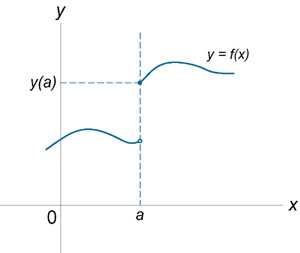
\includegraphics{img/fig1.jpg}
% \caption{Discontinuity}
% \end{figure}

% У заключения нет номера главы
\section*{Conclusion and future work}

\setmonofont[Mapping=tex-text]{CMU Typewriter Text}
% \pagenumbering{gobble}
% \bibliographystyle{plain}
% \bibliography{thesis}
\printbibliography
\end{document}
